\documentclass[12pt, titlepage]{article}

\usepackage{booktabs}
\usepackage{tabularx}
\usepackage{hyperref}
\usepackage[table,xcdraw]{xcolor}
\usepackage{longtable}
\usepackage{multirow}
\usepackage{graphicx}
\usepackage{float}
\hypersetup{
    colorlinks,
    citecolor=black,
    filecolor=black,
    linkcolor=red,
    urlcolor=blue
}
\usepackage[round]{natbib}

%% Comments

\usepackage{color}

\newif\ifcomments\commentstrue %displays comments
%\newif\ifcomments\commentsfalse %so that comments do not display

\ifcomments
\newcommand{\authornote}[3]{\textcolor{#1}{[#3 ---#2]}}
\newcommand{\todo}[1]{\textcolor{red}{[TODO: #1]}}
\else
\newcommand{\authornote}[3]{}
\newcommand{\todo}[1]{}
\fi

\newcommand{\wss}[1]{\authornote{blue}{SS}{#1}} 
\newcommand{\plt}[1]{\authornote{magenta}{TPLT}{#1}} %For explanation of the template
\newcommand{\an}[1]{\authornote{cyan}{Author}{#1}}

%% Common Parts

\newcommand{\progname}{ProgName} % PUT YOUR PROGRAM NAME HERE
\newcommand{\authname}{Team \#, Team Name
\\ Student 1 name
\\ Student 2 name
\\ Student 3 name
\\ Student 4 name} % AUTHOR NAMES                  

\usepackage{hyperref}
    \hypersetup{colorlinks=true, linkcolor=blue, citecolor=blue, filecolor=blue,
                urlcolor=blue, unicode=false}
    \urlstyle{same}
                                


\begin{document}

\title{Verification and Validation Report: \progname} 
\author{\authname}
\date{\today}
	
\maketitle

\pagenumbering{roman}

\section*{Revision History}

\begin{tabularx}{\textwidth}{p{3cm}p{2cm}X}
\toprule {\bf Date} & {\bf Version} & {\bf Notes}\\
\midrule
3/7/2023 & 1.0 & Added Section 1, 2, and 3 - Purpose, Scope, and Background\\
3/7/2023 & 1.1 & Added Section 4 - Functional Requirements Evaluation\\
3/7/2023 & 1.2 & Added Section 5 - Nonfunctional Requirements Evaluation\\
3/8/2023 & 1.3 & Added Section 6 - Unit Testing\\
\bottomrule
\end{tabularx}

\newpage

\tableofcontents

\listoftables

\newpage

\section*{Symbols, Abbreviations and Acronyms}


\renewcommand{\arraystretch}{1.2}
\begin{tabular}{l l} 
  \toprule		
  \textbf{symbol} & \textbf{description}\\
  \midrule 
  Age groups & (15-30, 31-50, 51-75, 75+)\\
  \bottomrule
\end{tabular}\\

\newpage

\pagenumbering{arabic}

\section{Purpose}

This VnV report's establishment is to support development of the product Synesthesia Wear. Furthermore, the actions taken in the document are linked with testing to ensure reliability and robustness of the product for adequate detection of particular sounds.

\section{Scope}

The focus of this document is on the output results of Synesthesia Wear when given arbitrary test inputs. Furthermore, black box testing will be used on important aspects of the output and input rather than how the results are being generated. Lastly, these tests will be based on certain implementations we have put into place to handle unexpected inputs.

\section{Background} 

Synesthesia wear is designed with a mobile application which allows customization to occur from their mobile devices and allows users to toggle certain sounds on and off to improve usability of the watch. Synesthesia wear will be able to detect key words and sounds that are customized to the users to aid them with their lack of hearing. As a result, this helps them know when someone is calling their name, during emergencies, and many other situations within their daily lives.


\section{Functional Requirements Evaluation}

\begin{longtable}{|p{1.4cm}|p{1cm}|p{3cm}|p{1.5cm}|p{2.5cm}|p{2cm}|p{1.2cm}|}

  \endfirsthead
  \endhead
  \hline
  \textbf{Id} & \textbf{Ref} & \textbf{Description}                                                         & \textbf{Input}                                    & \textbf{Expected Result}                                    & \textbf{Actual Result} & \textbf{Result}                                    \\ \hline
  FRT1        & FR1, FR2     & Testing ability to differentiate sounds                                     & Five different sounds                             & Device produces five different feedbacks                    &           Vibration motor was able to produce different feedbacks when configured with 5 different feedback settings              & {\color[HTML]{32CB00} Pass}                        \\ \hline
  FRT2        & FR1          & Testing in different environments                                            & Same sound in different environments              & Same feedback in all enviroments                            &          Feedback was the same in different environments              &         {\color[HTML]{32CB00} Pass}                \\ \hline
  FRT3        & FR1          & Testing at different ranges                                                  & Same sound at specified distances                 & Same feedback at specified distances                        &          Farther distances led to inconsistencies in the feedback              &  {\color[HTML]{FE0000} Fail} \\ \hline
  FRT4        & FR1          & Testing its ability to ignore ambient noise                                  & No input                                          & No output                                                   &          No vibrations are occuring when background noise is present in the environment              &       {\color[HTML]{32CB00} Pass}                                             \\ \hline
  FRT5        & FR2          & Testing its ability to classify correctly                                    & Different specified words                         & Feedback based on correct classification                    &          Feedback is correct with respect to the configured sound classification settings              &                    {\color[HTML]{32CB00} Pass}                               \\ \hline
  FRT6        & FR2          & Testing variability in speech                                                & Same word said by four different people           & Same feedback for all                                       &          Some inconsistencies in feedback for people with less training data samples               &            {\color[HTML]{FE0000} Fail}                                        \\ \hline
  FRT7        & FR2          & Testing its ability to ignore high amplitude random sounds                   & Random not specified sounds                       & No haptic feedback                                          &          No feedback occurred for the random sound samples              &                     {\color[HTML]{32CB00} Pass}                               \\ \hline
  FRT8        & FR3          & Testing newly set classifications                                            & A newly set classification sound                  & The specified haptic feedback                               &          The correct feedback for the newly configured sound occurred              &                  {\color[HTML]{32CB00} Pass}                                  \\ \hline
  FRT9        & FR3          & Testing removed classifications                                              & A removed classification sound                    & No feedback                                                 &          No feedback took place for the classification sound that was removed              &            {\color[HTML]{32CB00} Pass}                                        \\ \hline
  FRT10       & FR3          & Testing reboot and memory retention                                          & Power switched on and off and test FRT5 run again & Feedback based on correct classification                    &          Correct feedback still occurred after the device was rebooted              &               {\color[HTML]{32CB00} Pass}                                     \\ \hline
  FRT11       & FR4          & Testing haptic feedback with the device worn                                 & Specified sound                                   & Haptic feedback based on the sound's classification         &          The appropriate feedback happened even when the device was being worn              &                   {\color[HTML]{32CB00} Pass}                                 \\ \hline
  FRT12       & FR4          & Testing variability in haptic feedbacks                                      & Three different specified sounds                  & Different haptic feedbacks that convey the specified sounds &          Proper feedbacks with respect to each input sound occurred              &                              {\color[HTML]{32CB00} Pass}                      \\ \hline
  FRT13       & FR4          & Testing different wearable orientations                                      & FRT12 run on different orienations                & All orientations give consistent output                     &          The same feedback was present for any device orientation that was used              &                 {\color[HTML]{32CB00} Pass}                                   \\ \hline
  FRT14       & FR4          & Testing intensity of feedback wearing different clothes of varying thickness & FRT12 run on three different clothes              & All clothes give consistent results                         &          The thicker clothes lead to inconsistencies in feedback              &                      {\color[HTML]{FE0000} Fail}                              \\ \hline
  FRT15       & FR5          & Testing real-time application of device                                      & Specified sound                                   & Correct classification within one second                    &          Feedback had occurred within one second after an input sound had been said aloud              &                  {\color[HTML]{32CB00} Pass}                                  \\ \hline
  \caption{Functional Requirement Tests}
  \label{functionalRequirementTests}
\end{longtable}

\section{Nonfunctional Requirements Evaluation}

\subsection{Manual}
\begin{longtable}{|p{1.4cm}|p{1cm}|p{3cm}|p{1.5cm}|p{2.5cm}|p{2cm}|p{1.2cm}|}
 
  \endfirsthead
  \endhead
  \hline
  \textbf{Id} & \textbf{Ref} & \textbf{Description}                                                         & \textbf{Input}                                    & \textbf{Expected Result}                                    & \textbf{Actual Result} & \textbf{Result}                                    \\ \hline
  NFRT3        & NFR1          & Testing button functionality based on button colour                     & Open Application                 & Different coloured buttons perform different functionalities    & Buttons with similar colour performed similar functions                        & {\color[HTML]{32CB00} Pass}                        \\ \hline
  NFRT6        & NFR1          & Testing usability, accessability, findability of application and device                     & N/A                              & Achieve average score of 8 from 10 participants (rated out of 10)                           &                       &  \cellcolor[HTML]{FFFFFF}{\color[HTML]{F8A102} TBD}                       \\ \hline
  NFRT7        & NFR2          & Testing user interface's consistency in appearance                     & N/A                              & Achieve average score of 4 out of all questions from participants                       &                        & \cellcolor[HTML]{FFFFFF}{\color[HTML]{F8A102} TBD} \\ \hline
  NFRT12        & NFR4         & Testing ability to configure different keywords on application                    & Click keyword selection button   & Keyword configuration screen                                                   & Reached keyword configuration screen on application                     & {\color[HTML]{32CB00} Pass}                                                    \\ \hline
  NFRT13        & NFR4         & Testing ability to select language of use on application                  & Preferred Language               & Application translated to preferred language                  &                        &           \cellcolor[HTML]{FFFFFF}{\color[HTML]{F8A102} TBD}                                         \\ \hline
  NFRT14        & NFR4         & Testing ability to select language of use on already set-up device                      & Change Language                  & Application translated to chosen language                                      &                        &     \cellcolor[HTML]{FFFFFF}{\color[HTML]{F8A102} TBD}                                               \\ \hline
  NFRT15        & NFR4         & Testing accuracy of translated languages on application                  & Team translates manuals          & Translated manuals                                          &                        &            \cellcolor[HTML]{FFFFFF}{\color[HTML]{F8A102} TBD}                                        \\ \hline
  \caption{Manual Nonfunctional Requirement Tests}
  \label{manualNonfunctionalRequirementTests}
\end{longtable}

\subsection{Stress}
		
\begin{longtable}{|p{1.4cm}|p{1.4cm}|p{3cm}|p{1.5cm}|p{2.5cm}|p{2cm}|p{1.2cm}|}

  \endfirsthead
  \endhead
  \hline
  \textbf{Id} & \textbf{Ref} & \textbf{Description}                                                         & \textbf{Input}                                    & \textbf{Expected Result}    & \textbf{Actual Result}                          & \textbf{Result}                                     \\ \hline
  NFRT11        & NFR3          & Check if you can configure an unrecognizable keyword              & Unreco-gnizable keyword                          & Keyword not supported                      & Keyword not supported                         & {\color[HTML]{32CB00} Pass}                         \\ \hline
  NFRT24        & NFR11         & Feed 6 samples 50 times each with random noise added. Check if correctly classified 90 percent of the time           & Sound clips   & 90 percent correct classification        & 82 percent classification. See Figure \ref*{Histogram} in Appendix     & {\color[HTML]{FE0000} Fail}                           \\ \hline
  NFRT25        & NFR12         & Check the average battery life of the device by timing when 10 different device runs out of battery  & 10 fully charged devices   & Average battery life of 10 devices is more than 12 hours                   &                     &\cellcolor[HTML]{FFFFFF}{\color[HTML]{F8A102} TBD}                          \\ \hline
  NFRT29        & NFR16         & Checking the durability of the device including material wear, battery etc & Device  & Lifetime of device should be 5 years&          & \cellcolor[HTML]{FFFFFF}{\color[HTML]{F8A102} TBD}                        \\ \hline
  \caption{Stress Nonfunctional Requirement Tests}
  \label{stressNonfunctionalRequirementTests}
\end{longtable}
\subsection{Performance}


\begin{longtable}{|p{1.4cm}|p{1cm}|p{3cm}|p{1.5cm}|p{2.5cm}|p{2cm}|p{1.2cm}|}
  \endfirsthead
  \endhead
  \hline
  \textbf{Id} & \textbf{Ref} & \textbf{Description}                                                         & \textbf{Input}                                    & \textbf{Expected Result}    & \textbf{Actual Result}                          & \textbf{Result}                                     \\ \hline
  NFRT1        & NFR1          & Checking what the initial state of application is.              & Open Application                          & Home Page of Application                      & Home Page of Application                        & {\color[HTML]{32CB00} Pass}                         \\ \hline
  NFRT2        & NFR1          & Can users find the pairing button of the application.           & Open the Application, Click pair button   & User clicks pair button under 10 seconds      & Users found pairing buttons under 10 seconds    & {\color[HTML]{32CB00} Pass}                         \\ \hline
  NFRT4        & NFR1          & Checking if application correctly goes to pairing page.         & Open the Application, Click pair button   & Pairing page of Application                   & Pairing page of Application                     & {\color[HTML]{32CB00} Pass}                         \\ \hline
  NFRT5        & NFR1          & Checking if application correctly goes to keyword selection page.& Open the Application, Click keyword selection button.& Keyword Selection page of Application& Keyword Selection page of Application        & {\color[HTML]{32CB00} Pass}                         \\ \hline
  NFRT8        & NFR3          & Check to see if the application connects to the device through bluetooth& Open application, click pair button on both device and application&Device pairs to Phone&Device Pairs to Phone                       & {\color[HTML]{32CB00} Pass}                        \\ \hline
  NFRT16       & NFR5          & Checking if users can pair a device to phone in under 5 minutes  & Open application, click pair button on both device and application& 3/4 Users fully pair device in under 5 minutes& 4/4 Users pair device under 5 minutes&{\color[HTML]{32CB00} Pass}            \\ \hline
  NFRT19       & NFR9          & A sound will be fed to the device that includes a keyword device should be able to provide feedback in under 1 second 8/10 times& Sound that includes a keyword&8/10 keywords detected in under 1 second& 9/10 Keywords detected. See Figure \ref*{Response} in Appendix&{\color[HTML]{32CB00} Pass}         \\ \hline
  NFRT20       & NFR9          & Checking how fast the UI of application responds to user input   &User Input & Average of 100 inputs is under 1ms&                                                                                             & \cellcolor[HTML]{FFFFFF}{\color[HTML]{F8A102} TBD}  \\ \hline
  NFRT21       & NFR9          & Checking that application can separately connect to 5 independent devices&Pairing button on both application and device& 5/5 devices pair in under 1 minute & All 5 paired in under 1 minute each              &{\color[HTML]{32CB00} Pass}                          \\ \hline           
  NFRT30       & NFR17         & Let 10 people use device for 3 days record how many say it inhibits their lives &unpaired device and unopened application & 8/10 participants do not the device to inhibit their lives &                       &\cellcolor[HTML]{FFFFFF}{\color[HTML]{F8A102} TBD}    \\ \hline           
  NFRT32       & NFR17         & Check to see if users can install the application on IOS and Android& Click Install & installed application on IOS and Android&Installed on Android          &{\color[HTML]{FE0000} Fail}                                                       \\ \hline
  \caption{Performance Nonfunctional Requirement Tests}
  \label{performanceNonfunctionalRequirementTests}
\end{longtable}

\subsection{Security}

\begin{longtable}{|p{1.4cm}|p{1cm}|p{3cm}|p{1.5cm}|p{2.5cm}|p{2cm}|p{1.2cm}|}
  \endfirsthead
  \endhead
  \hline
  \textbf{Id} & \textbf{Ref} & \textbf{Description}                                                         & \textbf{Input}                                    & \textbf{Expected Result}    & \textbf{Actual Result}                          & \textbf{Result}                                     \\ \hline
  NFRT9        & NFR3          & Checking if application pairs to device that is not in pairing mode              & Click pair Button & Device not found & Device not found & {\color[HTML]{32CB00} Pass}                         \\ \hline
  NFRT10        & NFR3          & Check if user can Login to application without a registered account           & Invalid Login Credintials   &  Account not found      & Account not found    & {\color[HTML]{32CB00} Pass}                         \\ \hline
  \caption{Security Nonfunctional Requirement Tests}
  \label{securityNonfunctionalRequirementTests}
\end{longtable}

\subsection{Recovery}

\begin{longtable}{|p{1.4cm}|p{1cm}|p{3cm}|p{1.5cm}|p{2.5cm}|p{2cm}|p{1.2cm}|}
  \endfirsthead
  \endhead
  \hline
  \textbf{Id} & \textbf{Ref} & \textbf{Description}                                                         & \textbf{Input}                                    & \textbf{Expected Result}    & \textbf{Actual Result}                          & \textbf{Result}                                     \\ \hline
  NFRT18        & NFR8          & Check to see if a initially paired device will automatically repair when taken out of range than put back into range              & Take device in/out of range  & device should rapair 90 percent of the time   & device repaired 100 percent of the time    & {\color[HTML]{32CB00} Pass}                         \\ \hline
  NFRT22        & NFR9          & Checking to see how long it takes a paired device to repair when brough back into range.             & place device back into range    & Average time of reconnection should be 10 seconds or less          & Average time was 6 seconds       & {\color[HTML]{32CB00} Pass}                         \\ \hline
  \caption{Recovery Nonfunctional Requirement Tests}
  \label{RecoveryNonfunctionalRequirementTests}
\end{longtable}


\subsection{Visual}

\begin{longtable}{|p{1.4cm}|p{1.4cm}|p{3cm}|p{1.5cm}|p{2.5cm}|p{2cm}|p{1.2cm}|}
  \endfirsthead
  \endhead
  \hline
  \textbf{Id} & \textbf{Ref} & \textbf{Description}                                                         & \textbf{Input}                                    & \textbf{Expected Result}    & \textbf{Actual Result}                          & \textbf{Result}                                     \\ \hline
  NFRT17        &  NFR6         & people from different age groups will be shown icons found in application and asked if they can identify their meaning                   & N/A    & All 5 icons named by 3/4 participants of each age group    &    & \cellcolor[HTML]{FFFFFF}{\color[HTML]{F8A102} TBD}                         \\ \hline
  NFRT23        &  NFR10        & Check if battery is visual on the final device             & N/A      & Battery should not be visible          & Battery is not visible       & {\color[HTML]{32CB00} Pass}                         \\ \hline
  NFRT31        &  NFR17        & Check if the device is adjustable such that it fits on different sized wrists            & Adjust size      & Should fit wrists of size 6-8.5 inches          & Fits specified Wrist sizes       & {\color[HTML]{32CB00} Pass}                         \\ \hline
  NFRT34        &  NFR25        & Check if the code has anything that would be offensive to any groups             & N/A      & There should not be anything offensive present          & Nothing that is offensive was found       & {\color[HTML]{32CB00} Pass}                         \\ \hline
  \caption{Visual Nonfunctional Requirement Tests}
  \label{VisualNonfunctionalRequirementTests}
\end{longtable}


\subsection{Load}

\begin{longtable}{|p{1.4cm}|p{1.4cm}|p{3cm}|p{1.5cm}|p{2.5cm}|p{2cm}|p{1.2cm}|}

  \endfirsthead
  \endhead
  \hline
  \textbf{Id} & \textbf{Ref} & \textbf{Description}                                                         & \textbf{Input}                                    & \textbf{Expected Result}    & \textbf{Actual Result}                          & \textbf{Result}                                     \\ \hline
  NFRT26        & NFR12          & Device will be turned on for a duration of 5 hours during which keywords will be fed at randon time intervals. Test passes if device reacts at each interval                & Sound clips       & Device should react at each of teh 5 random intervals        & device reacts at 5/5 intervals      & {\color[HTML]{32CB00} Pass}                         \\ \hline
  \caption{Load Nonfunctional Requirement Tests}
  \label{LoadNonfunctionalRequirementTests}
\end{longtable}

\subsection{Regulation}

\begin{longtable}{|p{1.4cm}|p{1.4cm}|p{3cm}|p{1.5cm}|p{2.5cm}|p{2cm}|p{1.2cm}|}

  \endfirsthead
  \endhead
  \hline
  \textbf{Id} & \textbf{Ref} & \textbf{Description}                                                         & \textbf{Input}                                    & \textbf{Expected Result}    & \textbf{Actual Result}                          & \textbf{Result}                                     \\ \hline
  NFRT35        & NFR26          & Team of lawyers will check if the project as a whole corresponds with all legal rulations and requirements.                & N/A         & Project follows all legal requirements           &          & \cellcolor[HTML]{FFFFFF}{\color[HTML]{F8A102} TBD}                        \\ \hline
  \caption{Regulation Nonfunctional Requirement Tests}
  \label{RegulationNonfunctionalRequirementTests}
\end{longtable}

\subsection{Upgrade}

\begin{longtable}{|p{1.4cm}|p{1.4cm}|p{3cm}|p{1.5cm}|p{2.5cm}|p{2cm}|p{1.2cm}|}
  \endfirsthead
  \endhead
  \hline
  \textbf{Id} & \textbf{Ref} & \textbf{Description}                                                         & \textbf{Input}                                    & \textbf{Expected Result}    & \textbf{Actual Result}                          & \textbf{Result}                                     \\ \hline
  NFRT27        & NFR12          & Helper code will be used to check if application is currently up if application goes down the developers will recieve an email              & N/A         & Application should have a continous uptime of 1 year         &       & \cellcolor[HTML]{FFFFFF}{\color[HTML]{F8A102} TBD}                        \\ \hline
  NFRT28        & NFR15          & Check if products supports up to 10 keywords 2 years after launch.              & 10 keywords         & product will support at minimum 10 keywords         &       & \cellcolor[HTML]{FFFFFF}{\color[HTML]{F8A102} TBD}                        \\ \hline
  NFRT33        & NFR20          & Try and using the device 24 hours after a major update has been pushed to the application              & Input a sound         & Device should retain 100 percent functionality         &       & \cellcolor[HTML]{FFFFFF}{\color[HTML]{F8A102} TBD}                        \\ \hline
  \caption{Upgrade Nonfunctional Requirement Tests}
  \label{UpgradeNonfunctionalRequirementTests}
\end{longtable}


\section{Unit Testing}
The following test cases were derived from the unit test section shown in Synesthesia Wear's \href{https://github.com/jordanbierbrier/capstone/blob/main/docs/VnVPlan/VnVPlan.pdf}{\textit{VnVPlan.pdf Document}} as well as the modules shown in the \href{https://github.com/jordanbierbrier/capstone/blob/main/docs/Design/SoftDetailedDes/MIS.pdf}{\textit{MIS.pdf Document}}.
Furthermore, inapplicable tests from the VnVPlan were not included in the following table as they were not feasible with our current implementation.
\begin{longtable}{|p{1.4cm}|p{1cm}|p{3cm}|p{1.5cm}|p{2.5cm}|p{2cm}|p{1.2cm}|}

  \endfirsthead
  \endhead
  \hline
  \textbf{Id} & \textbf{Ref} & \textbf{Description}                                                         & \textbf{Input}                                    & \textbf{Expected Result}                                    & \textbf{Actual Result} & \textbf{Result}                                    \\ \hline
  UT1       &   M4, M9   & Testing accuracy of the microphone to detect sounds                                      & 3 Different Sample Recordings                             & 3 Distinct Sample Recordings in memory buffer that match the inputs respectively                    &     The detected sounds matched the input sounds                    & {\color[HTML]{32CB00} Pass} \\ \hline
  UT3       &   M8   & Testing bluetooth's ability to send signals accurately                                                  & Sample classification signal asserted on software                 & Feedback signal asserted on hardware                        &         According to the classification signal, the correct feedback signal was sent to the vibration motor               & {\color[HTML]{32CB00} Pass} \\ \hline
  UT4       &   M7   & Testing classification module's ability to accurately categorize sound data  & Stored samples of sound data in the memory buffer              & Accurately classified Sound Data                          &         The classification of the input sound samples were accurately categorized with a confidence level of 80\% or more               &                   {\color[HTML]{32CB00} Pass}                                 \\ \hline
  UT5       &   M7   & Testing classification module's ability to change its sound classification settings                                      & New Classification settings                                  & Classification settings have been changed on the app                    &       The settings displayed on the settings page match the newly inputted classification settings                 &       {\color[HTML]{32CB00} Pass}                                             \\ \hline
  UT6       &   M4, M7   & Testing feedback module's ability to transmit accurate feedback signals according to the settings  & Feedback signal is asserted              & Vibration detected in the bracelet that coincides with the feedback signal                          &      Vibration motor went off appropriately with respect to the settings configured on the app                        &   {\color[HTML]{32CB00} Pass}                    \\ \hline
  UT9       &   M2, M8   & Testing bluetooth connection ability                                     & Enable bluetooth connection                                  & Bluetooth connection connected in under a minute                    &         Bluetooth connection was established within 10 seconds               &             {\color[HTML]{32CB00} Pass}                                       \\ \hline
  UT10      &   M2, M9   & Testing bluetooth connection's ability when devices go in and out of range                                      & Separate the connected devices 10 or more metres away, wait at least 5 seconds, then bring the devices closer together                                  & Bluetooth will disconnect and reconnect when devices are back in range to each other                    &          Bluetooth was unable to automatically reconnect when devices went back in range            &                         {\color[HTML]{FE0000} Fail}                             \\ \hline
  UT11      &   M4   & Testing noise filtering module's ability to remove noise from a sample sound                                      & Digital data with one or more sounds                                  & Same digital sound recording but with less noise                    &          The output still had noise but notably less compared to the original sound file              &                    {\color[HTML]{32CB00} Pass}                                \\ \hline
  UT15      &   M5   & Testing app interface's ability to respond quickly to a user input                                      & User input                                  & User Interface response within 1ms                    &         The app was appropriately able to respond as soon as a button was clicked or an input was submitted               &                {\color[HTML]{32CB00} Pass}                                    \\ \hline
  UT16      &   M5   & Testing app interface's ability to respond the same across different systems (Android, Windows, IOS)                                      & User Input                                  & Same User Interface response on all the different devices                    &        N/A (The app has not yet been implemented on different IOS systems)                &                  \cellcolor[HTML]{FFFFFF}{\color[HTML]{F8A102} N/A}                                  \\ \hline
  \caption{Unit Tests}
  \label{unitTests}
\end{longtable}

\section{Changes Due to Testing}
Test results marked as {\color[HTML]{FE0000} Fail} require revisions in future implementations. 
\subsection{Changes Due to Requirement Tests}
\begin{itemize}
  \item Add capability to detect sounds at greater distance ($>$15m)
  \item Update sound detection model performance by being more generalizable (i.e. detect sound from different individuals) and have higher accuracy
\end{itemize}
\subsection{Changes Due to Unit Tests}
\begin{itemize}
  \item Add further bluetooth capability to reconnect device with mobile application after device goes in and out of range
\end{itemize}

\section{Traceability Matrices}
All of our tests can be traced back to either functional requirements, nonfunctional requirements and modules.
\begin{table}[H]
  \centering
  \begin{tabular}{|l|lllll|}
  \hline
  \textbf{Test}  & \multicolumn{5}{l|}{\textbf{Requirements}}                                                                                                                   \\ \hline
                 & \multicolumn{1}{l|}{\textbf{FR1}} & \multicolumn{1}{l|}{\textbf{FR2}} & \multicolumn{1}{l|}{\textbf{FR3}} & \multicolumn{1}{l|}{\textbf{FR4}} & \textbf{FR5} \\ \hline
  \textbf{FRT1}  & \multicolumn{1}{l|}{X}            & \multicolumn{1}{l|}{X}            & \multicolumn{1}{l|}{}             & \multicolumn{1}{l|}{}             &              \\ \hline
  \textbf{FRT2}  & \multicolumn{1}{l|}{X}            & \multicolumn{1}{l|}{}             & \multicolumn{1}{l|}{}             & \multicolumn{1}{l|}{}             &              \\ \hline
  \textbf{FRT3}  & \multicolumn{1}{l|}{X}            & \multicolumn{1}{l|}{}             & \multicolumn{1}{l|}{}             & \multicolumn{1}{l|}{}             &              \\ \hline
  \textbf{FRT4}  & \multicolumn{1}{l|}{X}            & \multicolumn{1}{l|}{}             & \multicolumn{1}{l|}{}             & \multicolumn{1}{l|}{}             &              \\ \hline
  \textbf{FRT5}  & \multicolumn{1}{l|}{}             & \multicolumn{1}{l|}{X}            & \multicolumn{1}{l|}{}             & \multicolumn{1}{l|}{}             &              \\ \hline
  \textbf{FRT6}  & \multicolumn{1}{l|}{}             & \multicolumn{1}{l|}{X}            & \multicolumn{1}{l|}{}             & \multicolumn{1}{l|}{}             &              \\ \hline
  \textbf{FRT7}  & \multicolumn{1}{l|}{}             & \multicolumn{1}{l|}{X}            & \multicolumn{1}{l|}{}             & \multicolumn{1}{l|}{}             &              \\ \hline
  \textbf{FRT8}  & \multicolumn{1}{l|}{}             & \multicolumn{1}{l|}{}             & \multicolumn{1}{l|}{X}            & \multicolumn{1}{l|}{}             &              \\ \hline
  \textbf{FRT9}  & \multicolumn{1}{l|}{}             & \multicolumn{1}{l|}{}             & \multicolumn{1}{l|}{X}            & \multicolumn{1}{l|}{}             &              \\ \hline
  \textbf{FRT10} & \multicolumn{1}{l|}{}             & \multicolumn{1}{l|}{}             & \multicolumn{1}{l|}{X}            & \multicolumn{1}{l|}{}             &              \\ \hline
  \textbf{FRT11} & \multicolumn{1}{l|}{}             & \multicolumn{1}{l|}{}             & \multicolumn{1}{l|}{}             & \multicolumn{1}{l|}{X}            &              \\ \hline
  \textbf{FRT12} & \multicolumn{1}{l|}{}             & \multicolumn{1}{l|}{}             & \multicolumn{1}{l|}{}             & \multicolumn{1}{l|}{X}            &              \\ \hline
  \textbf{FRT13} & \multicolumn{1}{l|}{}             & \multicolumn{1}{l|}{}             & \multicolumn{1}{l|}{}             & \multicolumn{1}{l|}{X}            &              \\ \hline
  \textbf{FRT14} & \multicolumn{1}{l|}{}             & \multicolumn{1}{l|}{}             & \multicolumn{1}{l|}{}             & \multicolumn{1}{l|}{X}            &              \\ \hline
  \textbf{FRT15} & \multicolumn{1}{l|}{}             & \multicolumn{1}{l|}{}             & \multicolumn{1}{l|}{}             & \multicolumn{1}{l|}{}             & X            \\ \hline
  \end{tabular}
  \caption{Traceability between functional requirement tests and functional requirements }
  \label{tab:my-table}
\end{table}

\noindent Given our size of non-functional requirements, we have grouped some of the tests into test types for ease of understanding.
% Please add the following required packages to your document preamble:
% \usepackage{multirow}
\begin{table}[H]
  \centering
  \begin{tabular}{|l|l|}
  \hline
  \textbf{Test Cases}                         & \textbf{Requirements} \\ \hline
  \multirow{3}{*}{Manual Non-functional}      & NFR1                  \\ \cline{2-2} 
                                              & NFR2                  \\ \cline{2-2} 
                                              & NFR4                  \\ \hline
  \multirow{4}{*}{Stress Non-functional}      & NFR3                  \\ \cline{2-2} 
                                              & NFR11                 \\ \cline{2-2} 
                                              & NFR12                 \\ \cline{2-2} 
                                              & NFR16                 \\ \hline
  \multirow{6}{*}{Performance Non-Functional} & NFR1                  \\ \cline{2-2} 
                                              & NFR3                  \\ \cline{2-2} 
                                              & NFR5                  \\ \cline{2-2} 
                                              & NFR9                  \\ \cline{2-2} 
                                              & NFR9                  \\ \cline{2-2} 
                                              & NFR17                 \\ \hline
  Security Non-Functional                                   & NFR3                  \\ \hline
  \end{tabular}
  \caption{Traceability between test cases and non-functional requirements }
  \label{tab:my-table}
\end{table}

\begin{table}[H]
  \centering
  \begin{tabular}{|p{2.5cm}|llllllllll|}
  \hline
  \textbf{Modules}                           & \multicolumn{10}{l|}{\textbf{Unit Tests}}                                                                                                                                                                                                                                                                                                  \\ \hline
                                              & \multicolumn{1}{l|}{\textbf{T1}} & \multicolumn{1}{l|}{\textbf{T3}} & \multicolumn{1}{l|}{\textbf{T4}} & \multicolumn{1}{l|}{\textbf{T5}} & \multicolumn{1}{l|}{\textbf{T6}} & \multicolumn{1}{l|}{\textbf{T9}} & \multicolumn{1}{l|}{\textbf{T10}} & \multicolumn{1}{l|}{\textbf{T11}} & \multicolumn{1}{l|}{\textbf{T15}} & \textbf{T16} \\ \hline
  \textbf{Login Module M1}                   & \multicolumn{1}{l|}{}            & \multicolumn{1}{l|}{}            & \multicolumn{1}{l|}{}            & \multicolumn{1}{l|}{}            & \multicolumn{1}{l|}{}            & \multicolumn{1}{l|}{}            & \multicolumn{1}{l|}{}             & \multicolumn{1}{l|}{}             & \multicolumn{1}{l|}{}             &              \\ \hline
  \textbf{Bluetooth connection Module M2}    & \multicolumn{1}{l|}{}            & \multicolumn{1}{l|}{}            & \multicolumn{1}{l|}{}            & \multicolumn{1}{l|}{}            & \multicolumn{1}{l|}{}            & \multicolumn{1}{l|}{X}           & \multicolumn{1}{l|}{X}            & \multicolumn{1}{l|}{}             & \multicolumn{1}{l|}{}             &              \\ \hline
  \textbf{Keyword Selection Module M3}       & \multicolumn{1}{l|}{}            & \multicolumn{1}{l|}{}            & \multicolumn{1}{l|}{}            & \multicolumn{1}{l|}{}            & \multicolumn{1}{l|}{}            & \multicolumn{1}{l|}{}            & \multicolumn{1}{l|}{}             & \multicolumn{1}{l|}{}             & \multicolumn{1}{l|}{}             &              \\ \hline
  \textbf{Output Signal Module M4}           & \multicolumn{1}{l|}{X}           & \multicolumn{1}{l|}{}            & \multicolumn{1}{l|}{}            & \multicolumn{1}{l|}{}            & \multicolumn{1}{l|}{X}           & \multicolumn{1}{l|}{}            & \multicolumn{1}{l|}{}             & \multicolumn{1}{l|}{X}            & \multicolumn{1}{l|}{}             &              \\ \hline
  \textbf{Profile Module M5}                 & \multicolumn{1}{l|}{}            & \multicolumn{1}{l|}{}            & \multicolumn{1}{l|}{}            & \multicolumn{1}{l|}{}            & \multicolumn{1}{l|}{}            & \multicolumn{1}{l|}{}            & \multicolumn{1}{l|}{}             & \multicolumn{1}{l|}{}             & \multicolumn{1}{l|}{X}            & X            \\ \hline
  \textbf{Battery Status Module M6}          & \multicolumn{1}{l|}{}            & \multicolumn{1}{l|}{}            & \multicolumn{1}{l|}{}            & \multicolumn{1}{l|}{}            & \multicolumn{1}{l|}{}            & \multicolumn{1}{l|}{}            & \multicolumn{1}{l|}{}             & \multicolumn{1}{l|}{}             & \multicolumn{1}{l|}{}             &              \\ \hline
  \textbf{Sound Classification Module M7}    & \multicolumn{1}{l|}{}            & \multicolumn{1}{l|}{}            & \multicolumn{1}{l|}{X}           & \multicolumn{1}{l|}{X}           & \multicolumn{1}{l|}{}            & \multicolumn{1}{l|}{}            & \multicolumn{1}{l|}{}             & \multicolumn{1}{l|}{}             & \multicolumn{1}{l|}{}             &              \\ \hline
  \textbf{Bluetooth Communication Module M8} & \multicolumn{1}{l|}{}            & \multicolumn{1}{l|}{X}           & \multicolumn{1}{l|}{}            & \multicolumn{1}{l|}{}            & \multicolumn{1}{l|}{X}           & \multicolumn{1}{l|}{X}           & \multicolumn{1}{l|}{}             & \multicolumn{1}{l|}{}             & \multicolumn{1}{l|}{}             &              \\ \hline
  \textbf{Microphone Module M9}              & \multicolumn{1}{l|}{X}           & \multicolumn{1}{l|}{}            & \multicolumn{1}{l|}{}            & \multicolumn{1}{l|}{}            & \multicolumn{1}{l|}{}            & \multicolumn{1}{l|}{}            & \multicolumn{1}{l|}{X}            & \multicolumn{1}{l|}{}             & \multicolumn{1}{l|}{}             &              \\ \hline
  \end{tabular}
  \caption{Traceability between modules and unit tests.}
  \label{tab:my-table}
\end{table}

\newpage{}
\section{Appendix}
\subsection{Test Results}
\subsection*{Response Time}
\begin{figure}[H]
  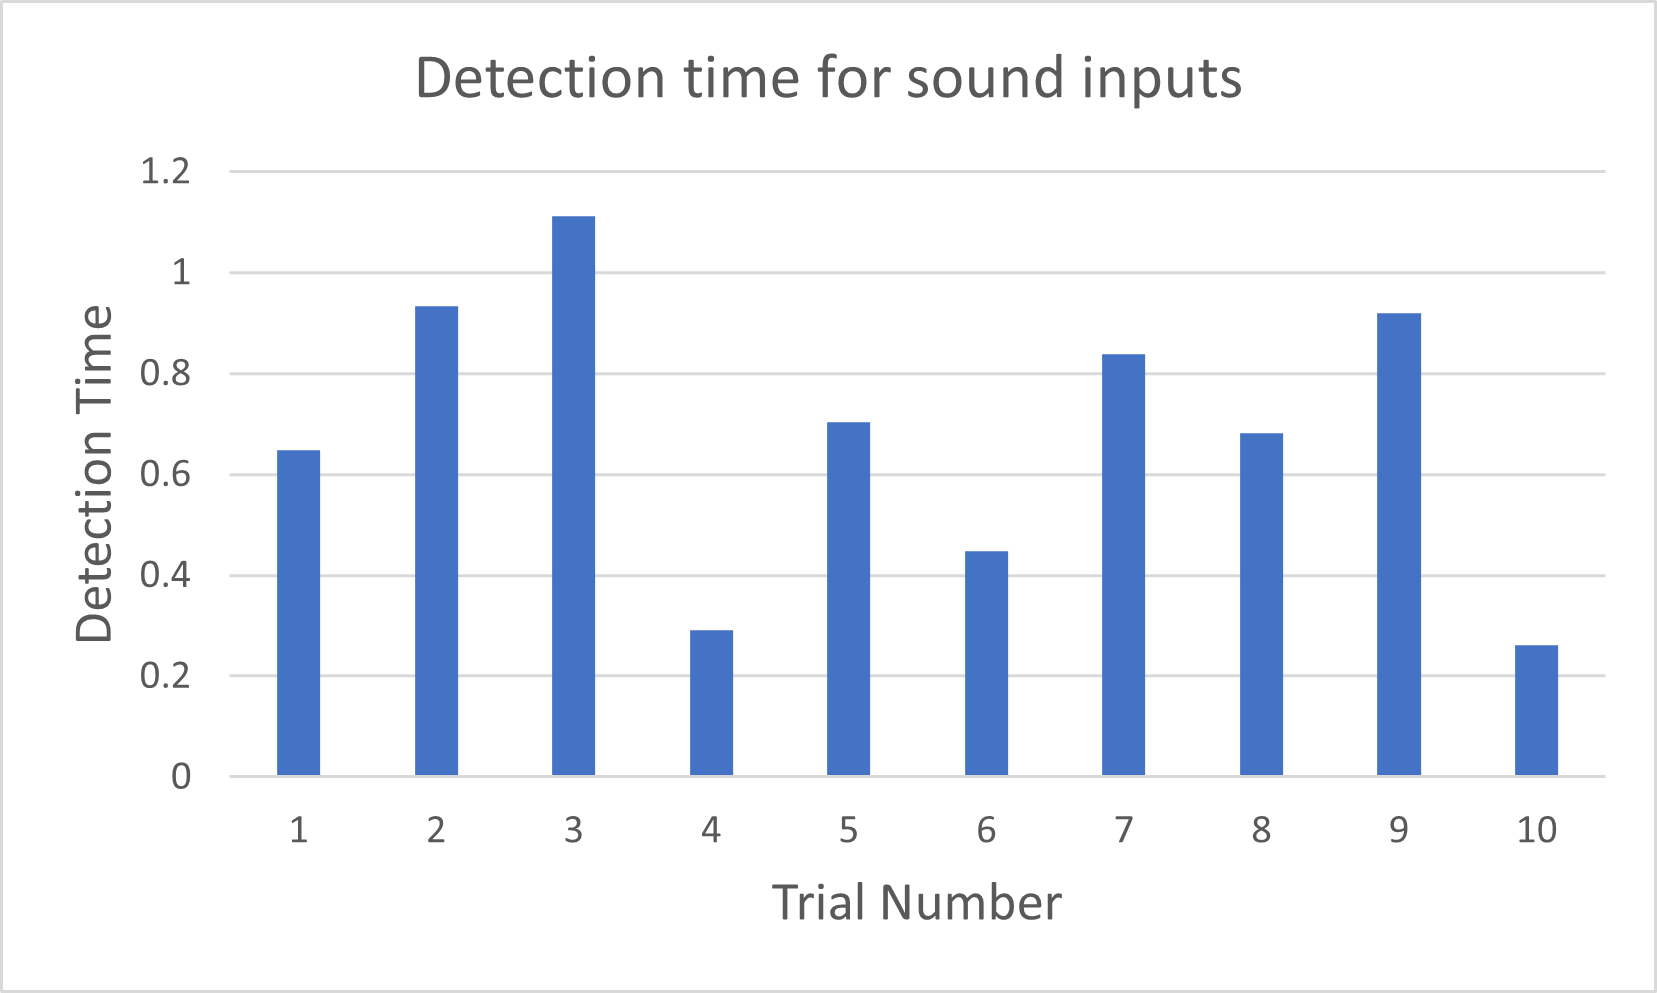
\includegraphics[width=\textwidth,height=\textheight,keepaspectratio]{Responce_time.png}
  \caption{Detection time for sound inputs}
  \label{Response} 
\end{figure}
\subsection*{Model Accuracy Histogram}
\begin{figure}[H]
  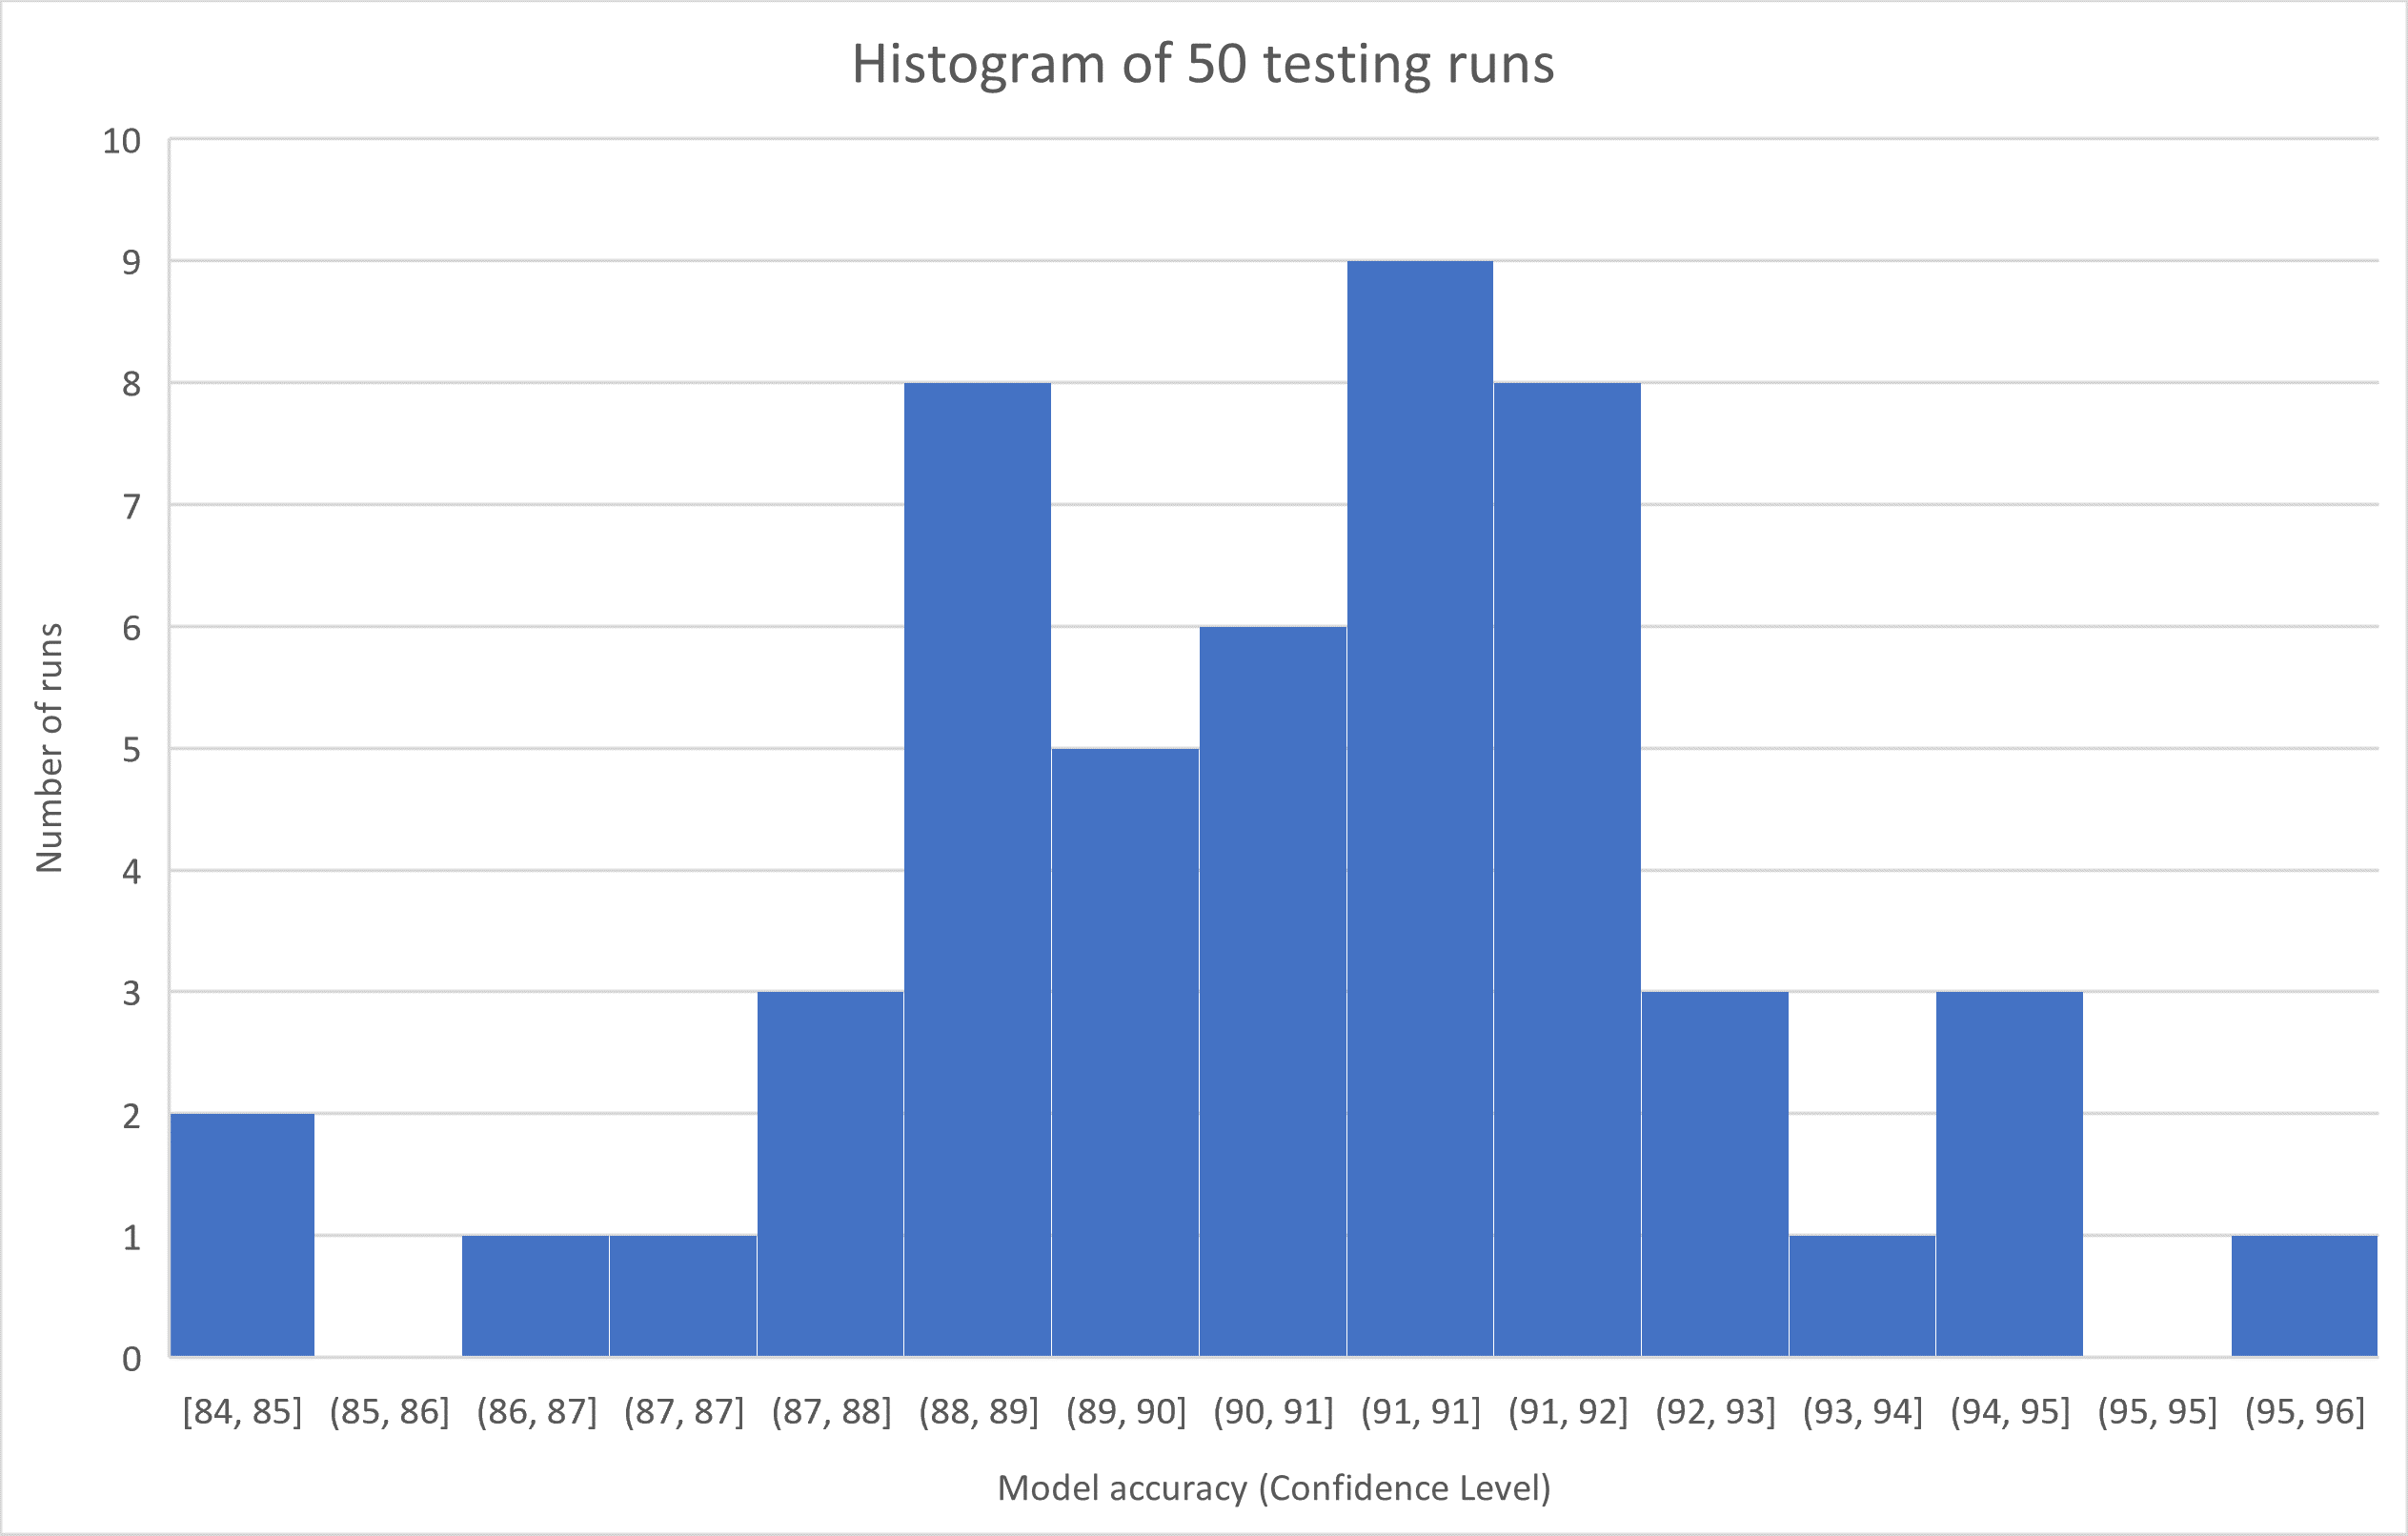
\includegraphics[width=\textwidth,height=\textheight,keepaspectratio]{confidence_level.png}
  \caption{Histogram of 50 testing runs}
  \label{Histogram} 
\end{figure}


\subsection{Reflection}

Reflecting on the VnV plan has showed difference between the predicted output in VnV plan compared to experimental ones found in the VnV report. This difference was still used to utilize our time effective by making the tests more concise and increase their usefulness. For example, a functional requirement test 3 is TBD in the VnV report compared to the predicted VnV plan which produces haptic feedback. 
\newline

\noindent Multiple other tests were founded to be based on reality which will be conducted after the final revision is completed. An example is NFRT 7, to test this we would need the finalized product design which would come later in the project to ensure no time is taken away from the usability of the device. 
\newline

\noindent To improve upon the differences between the two documents the team will collaboratively brainstorm ideas on every test and how it will conducted within the time frame given, rather then the unrealistic output of the devices. For example, testing an invalid keyword. Questions that we'd bring up would be, what would be considered an invalid keyword? Further, think about the consequences if the test fails and what the back up plan would be. Try looking for alternative options to get the desired output needed for the device to function as required.


\subsection{Synthesis}
To conduct our tests, data was required to be collected. Our functional requirement, nonfunctional requirement, and unit tests were carried out to determine the quality and effectiveness of our project. A majority of our tests passed, some were not able to be tested at this point in the development of our project. Additionally, a few tests failed. These are areas in which we will focus our next revision to improve. For example, we could make our sound classification model more robust, since the data we collected (experiments we ran) did not pass expected results. Overall, our goal is to have all of our test results as passes. 


\end{document}